% !TeX root = ../main.tex
\chapter{Parking Maneuver}\label{chapter:Parking Maneuver}
Various path planning algorithms have been presented for parking generation and steering motion. However, most of them are designed for a general motion of a robot or what is called \acrfull{clmr} \cite{CLMR}. These methods might not be usable for a real vehicle to produce a real time parking on streets. The assumption of most of these recent methods is that the actor(robot or car) is Non-holonomic which means there is no intolerable velocity constraint on vehicle \cite{parkingManeuver} i,e. Focus of these algorithms is to control the steering Angle and velocity of the vehicle or how to turn the steering to reach the expected point in a controlled speed. The method presented in \cite{parkingManeuver} has been chosen for our parking maneuver simulation. This method is based on the idea of sinusoidal control function \cite{sinusoids}. This approach is a feedback and planning method which means that motion control procedure is an iterative process which repeatedly localize the vehicle until a specified location of vehicle relative to its environment is reached. In the first iteration, vehicle enters to the parking place and gets a satisfied location compares to its environment but for optimizing the motion to set a perfect place in parking-bay where vehicle has the precise distance with adjacent cars and side of the parking-bay, this maneuver should be repeated in more iteration. iteration depends on the area of the parking-bay(its lateral and longitudinal measurements) and also size of the vehicle. This algorithm considers steering angle and velocity magnitudes as main maneuver parameters. Calculation of steering-angle and velocity depends on the calculation of the whole maneuvering time, maximum speed and maximum steering wheel of the vehicle which is applicable to the parking maneuver. It is obvious that this values depend on the model of the ego-vehicle, environment situation and also different simulators offer different values. Before calculating these main parameters of maneuver(speed and steering angle) and even before the calculation of maximum time, it is important to know the height and width of the parking bay and also size of the ego vehicle. According to above description, this parking maneuver algorithm could be classified as the following steps:
\begin{itemize}
\item Measurements of parking place(find longitudinal and lateral displacement)
\item Calculation of maximum values of maneuvering time(T$_{max}$) and steering   
angle($\Phi_{max}$) by evaluating vehicle model  which is explained in \ref{section: vehicle model}.
\item Steering vehicle based on the maximum values of the last step while processing the distances to other obstacles(like side of the parking and other vehicles) to prevent from collision
\item Check vehicle location relative to the environment and expected parked place and decide when to stop steering
\end{itemize}
In this work, as the detection of the parking place and setting the position of the vehicle has been done in the separate steps (in the last steps using machine learning algorithms), we made a little changes in the process of the algorithm. In our method, maximum time and steering angle is calculated just one time before the start of maneuver and after \ref{chapter: stabilization} but in \cite{parkingManeuver} this calculation is done before each iteration start. In the current project, we just made the maneuver in one iteration and as the vehicle reaches to the goal position in the first iteration we refused to make this movement iterative. However, to get an optimal position where vehicle has precise distance to the adjacent cars (say in the center of two vehicles) and also a satisfied distance to the sides of the parking-bay, this algorithm should be applied attractively with also some forward movement. In this project, the goal was to place the car inside of the parking without collision but for making a precise optimum location and as the goal was reached in the limited time of research, the other process of testing an iterative algorithm or making a nice position of the vehicle between two other cars, postponed to future works. calculation of maneuver parameters is based on the accurate kinematic and dynamic model of the vehicle. So next section provides an explanation of model and motion of the vehicle. Then base on this model, in \ref{section: calculation} section, a detail explanation of how T-max and Ø-max are calculated before start of parking motion has been provided and finally in \ref{section: motion} section, motion algorithm and how the vehicle is steered and moved to the parking-bay based on T-max and Ø-max values has been explained.
\begin{figure}
    \centering
    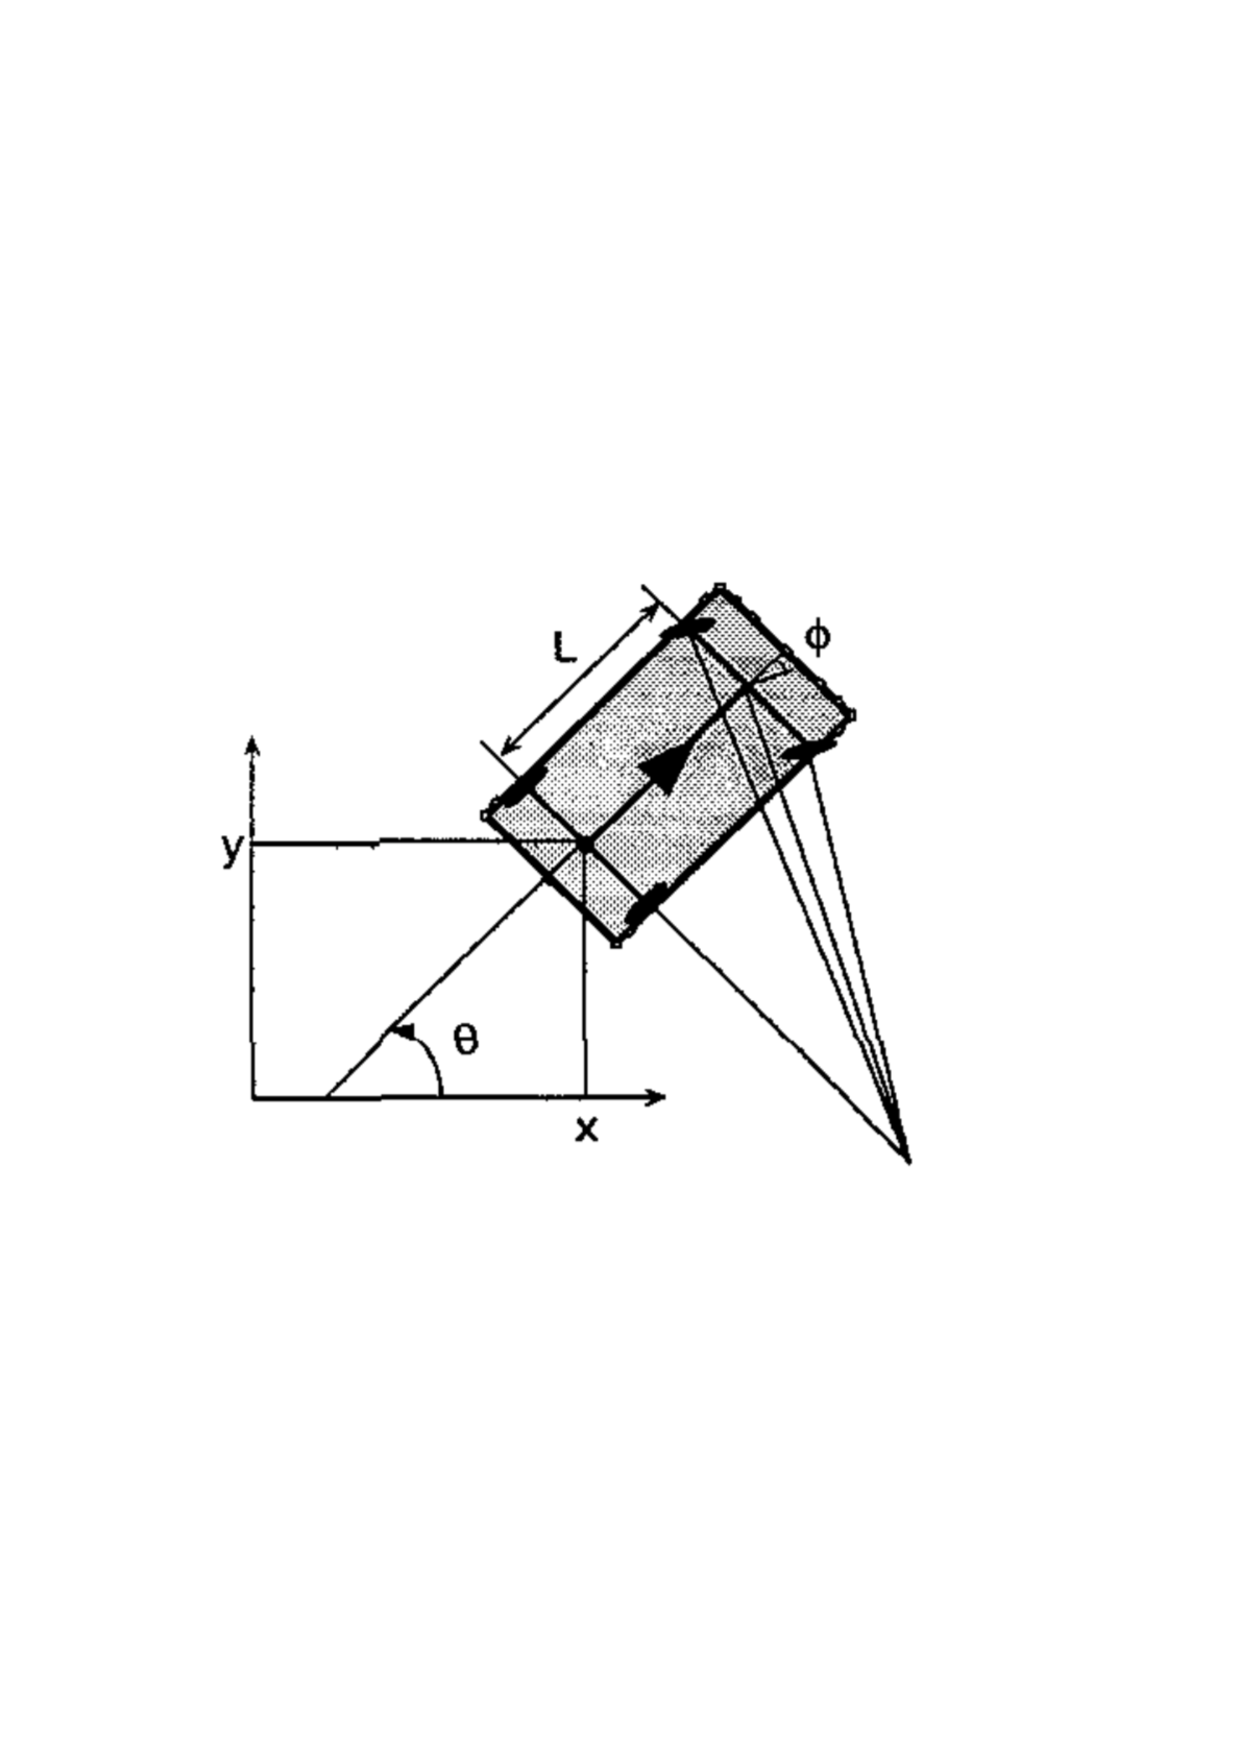
\includegraphics[width=9cm, height=4cm]{images/vehicleModel.pdf}
    \caption{Model of a non-holonomic vehicle \cite{parkingManeuver}}
    \label{fig:vehicleModel}
\end{figure}
\section{vehicle model} \label{section: vehicle model}
A four-wheeled vehicle model with its coordinates and steering can be seen in fig \ref{fig:vehicleModel}. As it can be seen vehicle's location described by three coordinates (x,y,$\theta$) where x and y are coordinates of the midpoint of vehicle's rear wheel and $\theta$ is the orientation angle of the vehicle. Motion of the vehicle can be described by following equations:
\begin{align} 
    \dot{x} = v \cdot cos(\phi) \cdot cos(\theta)\nonumber\\
	\dot{y} = v \cdot cos(\phi) \cdot sin(\theta)\nonumber\\
	\dot{\theta} = \frac{v}{L} \cdot sin(\phi)\label{eq2}
\end{align}
Where v refers to the longitudinal velocity, $\phi$ is the steering angle and L is a the wheel base and constant value referred to wheel base and can be defined in range 1.5 < L < 2 \cite{parkingManeuver}. This equation assumed that the vehicle is non-holonomic because using the derivatives of car's coordinate declared that these values are non-intolerable. Besides, these equations are valid for a vehicle which moves on a flat ground so they ignored the friction and slippage between the ground and vehicle's wheels. Future calculation of parking maneuver are based on this equations(of vehicle model) and as we know parallel parking movement affects on the lateral displacements of the vehicle into the parking-bay.
\section{Calculation} \label{section: calculation}
As already mentioned above, some calculation should be done before the start of the maneuver because to calculate the value of steering angle and velocity at each time of maneuver, the values of maximum steering and maximum time of maneuver should be known in advanced which also depends on the size/model of the car and environment situation like parking-bay's area so before going to the next section(motion phase), here an explanation of how this maximum values are calculated before start of the maneuver.
\subsection{Maneuver Time Calculation} \label{section: T-max}
Before starting the calculation of steering angle and velocity for parking maneuver (\ref{section: motion}), we should know the duration of whole parking maneuver. Computation of T is an iterative process based on the evaluation of vehicle's motion (\ref{eq2}). The idea is to change the values of x and y (location of the vehicle) in the path of the parking-bay to estimate the duration of passing parking area. To this end, values of x and y should be changed in an iterative process. Following constraint should be satisfied during these iterations.
\begin{align}
|(x_T-x_0)\cdot\cos{\theta_0}+(y_T-y_0)\cdot\sin{\theta_0}| < D_l
\end{align}\label{constraint1}
D$_l$ is the longitudinal displacement for the car in the parking-bay or length of the parking place and in each iteration, this constraint should be checked besides the value of $\Delta$T is added to the T value in each time (starts from 0). $\Delta$T is the sampling period of the movement which depends on the maneuver's speed and in simulation depends on the simulator and its sampling-rate. The calculation process also depends on the changes of steering angle and velocity at each time as their equations have been defined in the next section\ref{section: motion}. Based on the \ref{eq2}, the changes in x and y for each iteration is defined as follows:$\\$
When $\phi(t_n)=0$:
\begin{align} 
    \theta(t_n)=\theta(t_n-1)\nonumber\\
     x(t_n)=x(t_n-1)+v(t_n)\Delta T\cos{\theta(t_n)}\nonumber\\
	 y(t_n)=y(t_n-1)+v(t_n)\Delta T\sin{\theta(t_n)}\nonumber
\end{align}
and when $\phi(t_n)$ is not $0$:
\begin{align} 
     \theta(t_n)=\theta(t_n-1)+\frac{v(t_n)\Delta T}{L} sin\phi(t_n)\nonumber\\
     x(t_n)=x(t_n-1)+\frac{L}{tan\phi(t_n)} [ \sin{\theta(t_n)}-\sin{\theta(t_n-1)}]\nonumber\\
	     y(t_n)=y(t_n-1)+\frac{L}{tan\phi(t_n)} [ \cos{\theta(t_n)}-\cos{\theta(t_n-1)}]\label{coordinates' values}
\end{align}
So in each iteration, x and y is calculated according to the following equations and their values compared to the constraint(\ref{constraint1}) plus magnitude of T is increased by $\Delta$T. when the constraint is violated, iteration will be stopped and the value of T is returned as the maximum duration of parking maneuver (T$_{max}$) to the next step.
\subsection{Steering Angle Calculation} \label{section: steeringAngle}
Calculation of $\Phi_{max}$ is pretty similar to T$_{max}$. This is also an iterative process where values of $\Phi$ is started from an empirical value of steering angle which is the maximum magnitude of steering angle that vehicle's wheels could get and that depends on the model of the vehicle and again simulator. $\Phi$ value is reduced during the iteration till the following constraint is satisfied. Here we consider lateral displacement of parking and $\Phi$ value is reduced by $\Delta\Phi$ in each iteration till the lateral constraint is satisfied and in that time the last value of $\Phi$ is given as the maximum steering angle for the maneuver. 
\begin{align}
|(x_0-x_T)\cdot\sin{\theta_0}+(y_T-y_0)\cdot\cos{\theta_0}| < D_w
\end{align}\label{constraint2}
D$_w$ is the lateral displacement or width of the detected parking-bay.$\\$
Calculation of x and y c as the same for T calculation process.(\ref{coordinates' values})
\section{Motion phase} \label{section: motion}
After preparing all of the values which are required for maneuver and getting knowledge about parking bay and distances, vehicle should be moved to the parking-bay. As already mentioned above the parking movement in our applied method is based on steering the wheels of the vehicle in an appropriate velocity so here there are two calculations(speed and steering angle). These calculations are done during the maneuver. In other words, vehicle is steered till it reached a satisfied place inside the parking-bay. for setting the values of steering and velocity at each time of maneuver, these equations have been used \cite{parkingManeuver}. 
\begin{align}
    \phi(t) = \phi_{max} \cdot k_{\phi} \cdot A(t), \qquad 0\leq t < T \\
     v(t) = v_{max} \cdot k_v \cdot B(t), \qquad  0\leq t < T
\end{align}
As it can be seen from these equations maneuver started from time of 0 (t=0) and maximum period of maneuvering is T which is calculated in advance \ref{section: T-max}. In each time of maneuver new values for $\phi$ and v are set to the vehicle. $\Phi_{max}$ is what explained in \ref{section: steeringAngle}. v$_{max}$ is the maximum speed that a vehicle can get and again depends on the vehicle's model as well as environment situation which is also an empirical value during calculation. coefficient k$_{\phi}$ in steering angle calculation regards to the movement direction which is +1 when vehicle should be moved to the right side and -1 when it moves to the left.(depends on the parking situation) and k$_{v}$ in velocity calculation refers to the forward or backward movement(+1 for forward and -1 for backward). $A(t)$ and $B(t)$ functions are calculated as follows:
\begin{align}
    A(t) = \begin{cases}
					1, \hspace*{3,2cm} 0 \leq t < t'\\
					cos(\frac{\pi(t-t')}{T^*}), \hspace*{1,5cm} t' \leq t \leq T-t'\\
					-1, \hspace*{2,9cm} T-t' < t \leq T\\
				  \end{cases}\\ \nonumber\\
				  B(t) = 0.5 \cdot (1 - cos(\frac{4\pi t}{T})), \hspace*{0,6cm} 0 \leq t \leq T
\end{align}
As we see their calculation depends on $T^*$ which is maneuvering time for a one complete turn or the time that would take for vehicle to turn from $-\Phi_{max}$ to $+\Phi_{max}$. $t'$ is defined as: $t'= \frac{T-T^*}{2}, T^*<T$
\subsection{End of Maneuver}
In this approach time of the whole maneuver T$_max$ is estimated in advance but this is the estimation and it is also considered as a constraint for the maximum time of maneuver so to the stop time of maneuver should have also other constraints. In the presented work, distance of the vehicle to the backward obstacle (or other parked) vehicle and also lateral distances to the side of the parking are also checked during the maneuver and when vehicle reached to the satisfied distance from the rear vehicle, it should be stopped and situation considered as parked situation. In addition, to make sure that is a safe maneuver(collision-free), distances from all sides of the vehicle to other obstacles should be checked during maneuver and when the vehicle is about to contact with other vehicles or obstacle, it should be stopped and maneuver start again by positioning the vehicle to the first location. This is also explained in detail in the next chapter.

